\documentclass[1p]{elsarticle_modified}
%\bibliographystyle{elsarticle-num}

%\usepackage[colorlinks]{hyperref}
%\usepackage{abbrmath_seonhwa} %\Abb, \Ascr, \Acal ,\Abf, \Afrak
\usepackage{amsfonts}
\usepackage{amssymb}
\usepackage{amsmath}
\usepackage{amsthm}
\usepackage{scalefnt}
\usepackage{amsbsy}
\usepackage{kotex}
\usepackage{caption}
\usepackage{subfig}
\usepackage{color}
\usepackage{graphicx}
\usepackage{xcolor} %% white, black, red, green, blue, cyan, magenta, yellow
\usepackage{float}
\usepackage{setspace}
\usepackage{hyperref}

\usepackage{tikz}
\usetikzlibrary{arrows}

\usepackage{multirow}
\usepackage{array} % fixed length table
\usepackage{hhline}

%%%%%%%%%%%%%%%%%%%%%
\makeatletter
\renewcommand*\env@matrix[1][\arraystretch]{%
	\edef\arraystretch{#1}%
	\hskip -\arraycolsep
	\let\@ifnextchar\new@ifnextchar
	\array{*\c@MaxMatrixCols c}}
\makeatother %https://tex.stackexchange.com/questions/14071/how-can-i-increase-the-line-spacing-in-a-matrix
%%%%%%%%%%%%%%%

\usepackage[normalem]{ulem}

\newcommand{\msout}[1]{\ifmmode\text{\sout{\ensuremath{#1}}}\else\sout{#1}\fi}
%SOURCE: \msout is \stkout macro in https://tex.stackexchange.com/questions/20609/strikeout-in-math-mode

\newcommand{\cancel}[1]{
	\ifmmode
	{\color{red}\msout{#1}}
	\else
	{\color{red}\sout{#1}}
	\fi
}

\newcommand{\add}[1]{
	{\color{blue}\uwave{#1}}
}

\newcommand{\replace}[2]{
	\ifmmode
	{\color{red}\msout{#1}}{\color{blue}\uwave{#2}}
	\else
	{\color{red}\sout{#1}}{\color{blue}\uwave{#2}}
	\fi
}

\newcommand{\Sol}{\mathcal{S}} %segment
\newcommand{\D}{D} %diagram
\newcommand{\A}{\mathcal{A}} %arc


%%%%%%%%%%%%%%%%%%%%%%%%%%%%%5 test

\def\sl{\operatorname{\textup{SL}}(2,\Cbb)}
\def\psl{\operatorname{\textup{PSL}}(2,\Cbb)}
\def\quan{\mkern 1mu \triangleright \mkern 1mu}

\theoremstyle{definition}
\newtheorem{thm}{Theorem}[section]
\newtheorem{prop}[thm]{Proposition}
\newtheorem{lem}[thm]{Lemma}
\newtheorem{ques}[thm]{Question}
\newtheorem{cor}[thm]{Corollary}
\newtheorem{defn}[thm]{Definition}
\newtheorem{exam}[thm]{Example}
\newtheorem{rmk}[thm]{Remark}
\newtheorem{alg}[thm]{Algorithm}

\newcommand{\I}{\sqrt{-1}}
\begin{document}

%\begin{frontmatter}
%
%\title{Boundary parabolic representations of knots up to 8 crossings}
%
%%% Group authors per affiliation:
%\author{Yunhi Cho} 
%\address{Department of Mathematics, University of Seoul, Seoul, Korea}
%\ead{yhcho@uos.ac.kr}
%
%
%\author{Seonhwa Kim} %\fnref{s_kim}}
%\address{Center for Geometry and Physics, Institute for Basic Science, Pohang, 37673, Korea}
%\ead{ryeona17@ibs.re.kr}
%
%\author{Hyuk Kim}
%\address{Department of Mathematical Sciences, Seoul National University, Seoul 08826, Korea}
%\ead{hyukkim@snu.ac.kr}
%
%\author{Seokbeom Yoon}
%\address{Department of Mathematical Sciences, Seoul National University, Seoul, 08826,  Korea}
%\ead{sbyoon15@snu.ac.kr}
%
%\begin{abstract}
%We find all boundary parabolic representation of knots up to 8 crossings.
%
%\end{abstract}
%\begin{keyword}
%    \MSC[2010] 57M25 
%\end{keyword}
%
%\end{frontmatter}

%\linenumbers
%\tableofcontents
%
\newcommand\colored[1]{\textcolor{white}{\rule[-0.35ex]{0.8em}{1.4ex}}\kern-0.8em\color{red} #1}%
%\newcommand\colored[1]{\textcolor{white}{ #1}\kern-2.17ex	\textcolor{white}{ #1}\kern-1.81ex	\textcolor{white}{ #1}\kern-2.15ex\color{red}#1	}

{\Large $\underline{12a_{0794}~(K12a_{0794})}$}

\setlength{\tabcolsep}{10pt}
\renewcommand{\arraystretch}{1.6}
\vspace{1cm}\begin{tabular}{m{100pt}>{\centering\arraybackslash}m{274pt}}
\multirow{5}{120pt}{
	\centering
	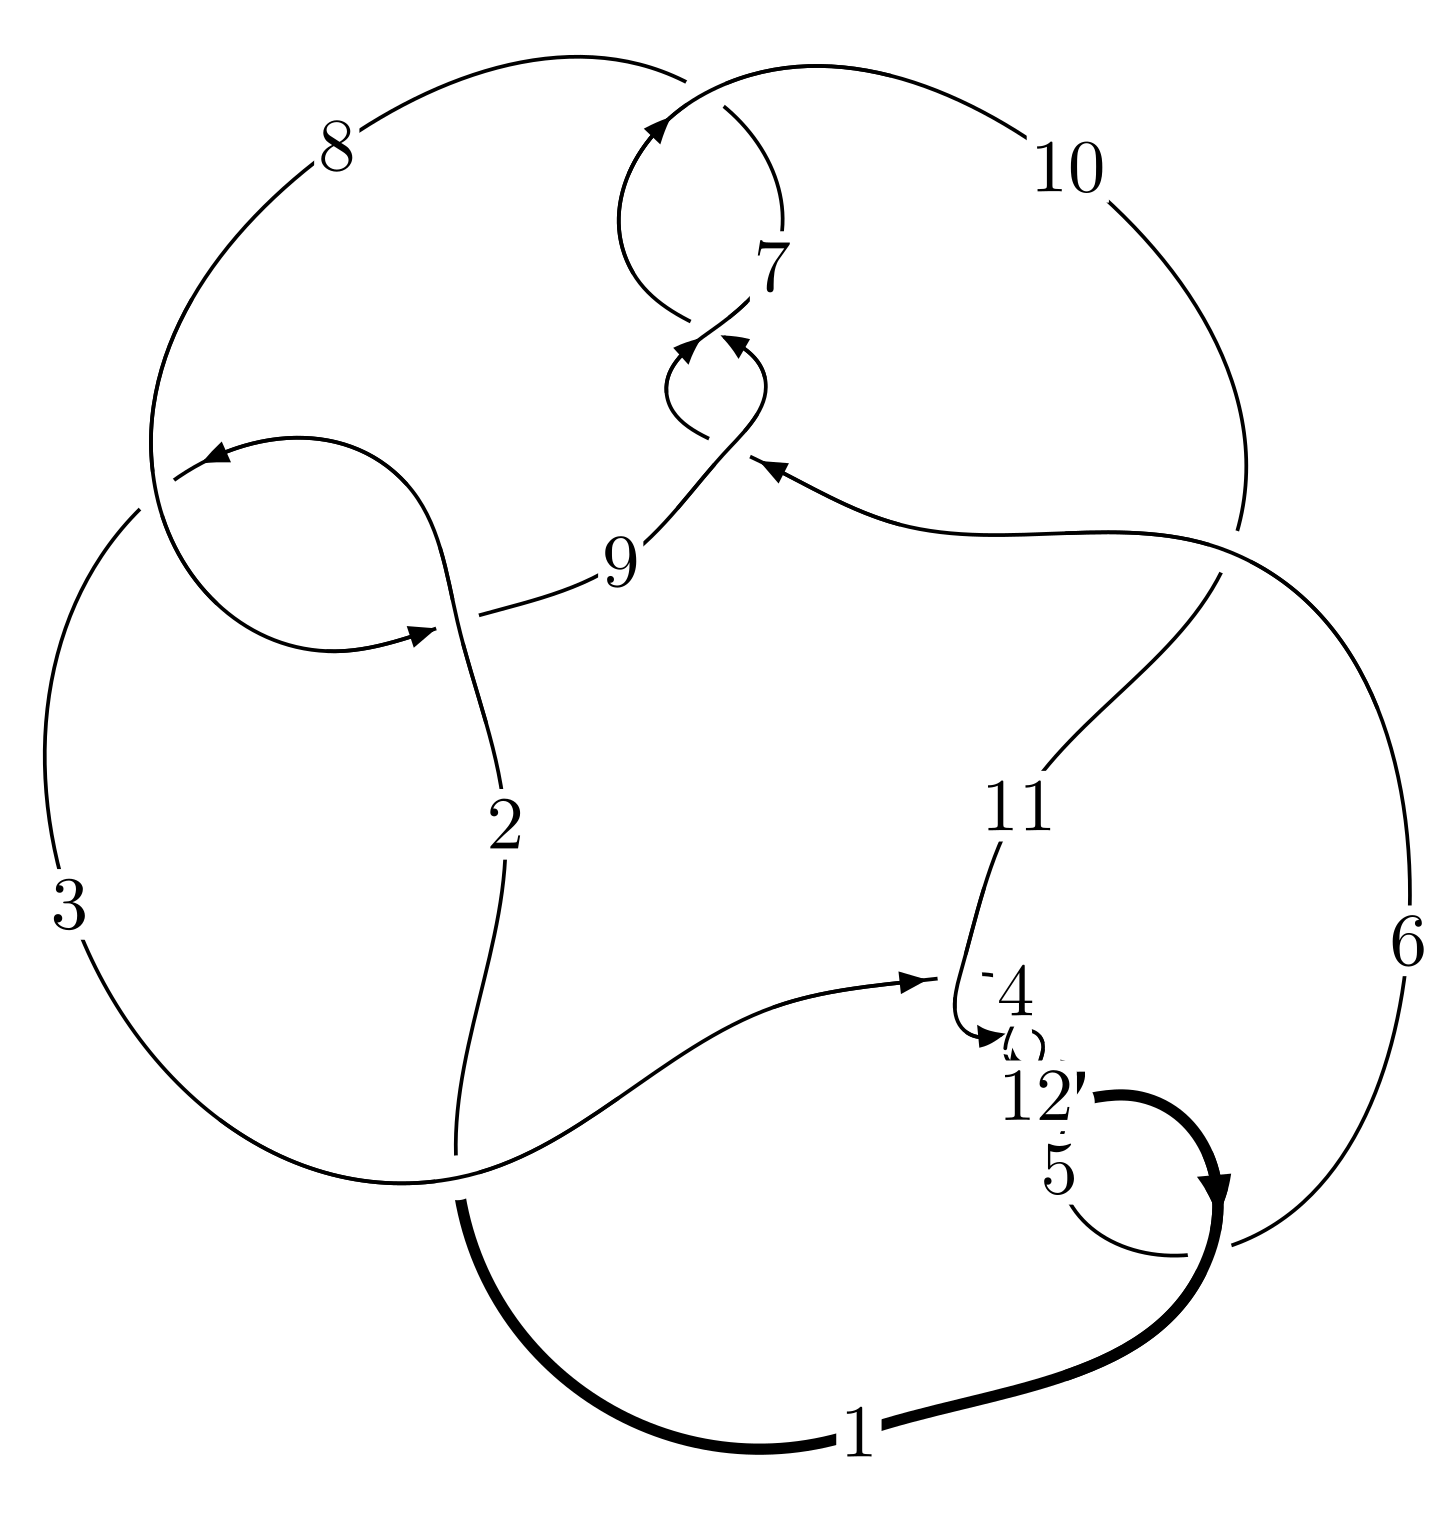
\includegraphics[width=112pt]{../../../GIT/diagram.site/Diagrams/png/1595_12a_0794.png}\\
\ \ \ A knot diagram\footnotemark}&
\allowdisplaybreaks
\textbf{Linearized knot diagam} \\
\cline{2-2}
 &
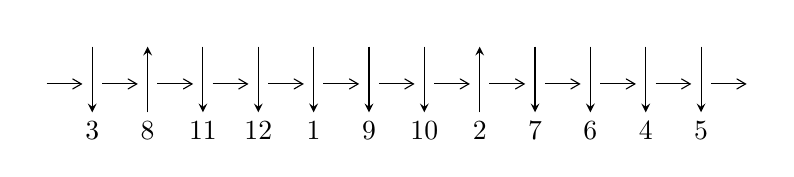
\begin{tikzpicture}[x=20pt, y=17pt]
	% nodes
	\node (C0) at (0, 0) {};
	\node (C1) at (1, 0) {};
	\node (C1U) at (1, +1) {};
	\node (C1D) at (1, -1) {3};

	\node (C2) at (2, 0) {};
	\node (C2U) at (2, +1) {};
	\node (C2D) at (2, -1) {8};

	\node (C3) at (3, 0) {};
	\node (C3U) at (3, +1) {};
	\node (C3D) at (3, -1) {11};

	\node (C4) at (4, 0) {};
	\node (C4U) at (4, +1) {};
	\node (C4D) at (4, -1) {12};

	\node (C5) at (5, 0) {};
	\node (C5U) at (5, +1) {};
	\node (C5D) at (5, -1) {1};

	\node (C6) at (6, 0) {};
	\node (C6U) at (6, +1) {};
	\node (C6D) at (6, -1) {9};

	\node (C7) at (7, 0) {};
	\node (C7U) at (7, +1) {};
	\node (C7D) at (7, -1) {10};

	\node (C8) at (8, 0) {};
	\node (C8U) at (8, +1) {};
	\node (C8D) at (8, -1) {2};

	\node (C9) at (9, 0) {};
	\node (C9U) at (9, +1) {};
	\node (C9D) at (9, -1) {7};

	\node (C10) at (10, 0) {};
	\node (C10U) at (10, +1) {};
	\node (C10D) at (10, -1) {6};

	\node (C11) at (11, 0) {};
	\node (C11U) at (11, +1) {};
	\node (C11D) at (11, -1) {4};

	\node (C12) at (12, 0) {};
	\node (C12U) at (12, +1) {};
	\node (C12D) at (12, -1) {5};
	\node (C13) at (13, 0) {};

	% arrows
	\draw[->,>={angle 60}]
	(C0) edge (C1) (C1) edge (C2) (C2) edge (C3) (C3) edge (C4) (C4) edge (C5) (C5) edge (C6) (C6) edge (C7) (C7) edge (C8) (C8) edge (C9) (C9) edge (C10) (C10) edge (C11) (C11) edge (C12) (C12) edge (C13) ;	\draw[->,>=stealth]
	(C1U) edge (C1D) (C2D) edge (C2U) (C3U) edge (C3D) (C4U) edge (C4D) (C5U) edge (C5D) (C6U) edge (C6D) (C7U) edge (C7D) (C8D) edge (C8U) (C9U) edge (C9D) (C10U) edge (C10D) (C11U) edge (C11D) (C12U) edge (C12D) ;
	\end{tikzpicture} \\
\hhline{~~} \\& 
\textbf{Solving Sequence} \\ \cline{2-2} 
 &
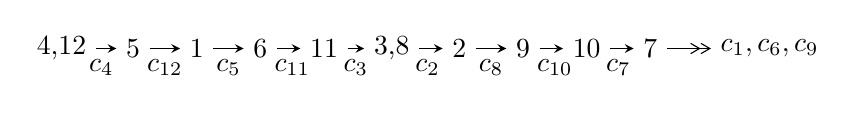
\begin{tikzpicture}[x=23pt, y=7pt]
	% node
	\node (A0) at (-1/8, 0) {4,12};
	\node (A1) at (1, 0) {5};
	\node (A2) at (2, 0) {1};
	\node (A3) at (3, 0) {6};
	\node (A4) at (4, 0) {11};
	\node (A5) at (81/16, 0) {3,8};
	\node (A6) at (49/8, 0) {2};
	\node (A7) at (57/8, 0) {9};
	\node (A8) at (65/8, 0) {10};
	\node (A9) at (73/8, 0) {7};
	\node (C1) at (1/2, -1) {$c_{4}$};
	\node (C2) at (3/2, -1) {$c_{12}$};
	\node (C3) at (5/2, -1) {$c_{5}$};
	\node (C4) at (7/2, -1) {$c_{11}$};
	\node (C5) at (9/2, -1) {$c_{3}$};
	\node (C6) at (45/8, -1) {$c_{2}$};
	\node (C7) at (53/8, -1) {$c_{8}$};
	\node (C8) at (61/8, -1) {$c_{10}$};
	\node (C9) at (69/8, -1) {$c_{7}$};
	\node (A10) at (11, 0) {$c_{1},c_{6},c_{9}$};

	% edge
	\draw[->,>=stealth]	
	(A0) edge (A1) (A1) edge (A2) (A2) edge (A3) (A3) edge (A4) (A4) edge (A5) (A5) edge (A6) (A6) edge (A7) (A7) edge (A8) (A8) edge (A9) ;
	\draw[->>,>={angle 60}]	
	(A9) edge (A10);
\end{tikzpicture} \\ 

\end{tabular} \\

\footnotetext{
The image of knot diagram is generated by the software ``\textbf{Draw programme}" developed by Andrew Bartholomew(\url{http://www.layer8.co.uk/maths/draw/index.htm\#Running-draw}), where we modified some parts for our purpose(\url{https://github.com/CATsTAILs/LinksPainter}).
}\phantom \\ \newline 
\centering \textbf{Ideals for irreducible components\footnotemark of $X_{\text{par}}$} 
 
\begin{align*}
I^u_{1}&=\langle 
- u^{41}+25 u^{39}+\cdots+b- u,\;u^{45}+u^{44}+\cdots+a+1,\;u^{47}+2 u^{46}+\cdots-2 u-1\rangle \\
I^u_{2}&=\langle 
b+u,\;a+1,\;u^2- u-1\rangle \\
\\
\end{align*}
\raggedright * 2 irreducible components of $\dim_{\mathbb{C}}=0$, with total 49 representations.\\
\footnotetext{All coefficients of polynomials are rational numbers. But the coefficients are sometimes approximated in decimal forms when there is not enough margin.}
\newpage
\renewcommand{\arraystretch}{1}
\centering \section*{I. $I^u_{1}= \langle - u^{41}+25 u^{39}+\cdots+b- u,\;u^{45}+u^{44}+\cdots+a+1,\;u^{47}+2 u^{46}+\cdots-2 u-1 \rangle$}
\flushleft \textbf{(i) Arc colorings}\\
\begin{tabular}{m{7pt} m{180pt} m{7pt} m{180pt} }
\flushright $a_{4}=$&$\begin{pmatrix}1\\0\end{pmatrix}$ \\
\flushright $a_{12}=$&$\begin{pmatrix}0\\u\end{pmatrix}$ \\
\flushright $a_{5}=$&$\begin{pmatrix}1\\u^2\end{pmatrix}$ \\
\flushright $a_{1}=$&$\begin{pmatrix}- u\\- u^3+u\end{pmatrix}$ \\
\flushright $a_{6}=$&$\begin{pmatrix}- u^2+1\\- u^4+2 u^2\end{pmatrix}$ \\
\flushright $a_{11}=$&$\begin{pmatrix}u\\u\end{pmatrix}$ \\
\flushright $a_{3}=$&$\begin{pmatrix}- u^2+1\\- u^2\end{pmatrix}$ \\
\flushright $a_{8}=$&$\begin{pmatrix}- u^{45}- u^{44}+\cdots-9 u-1\\u^{41}-25 u^{39}+\cdots+8 u^2+u\end{pmatrix}$ \\
\flushright $a_{2}=$&$\begin{pmatrix}u^7-4 u^5+4 u^3-2 u\\u^7-3 u^5+u\end{pmatrix}$ \\
\flushright $a_{9}=$&$\begin{pmatrix}-2 u^{46}- u^{45}+\cdots-20 u^2-7 u\\-2 u^{46}+58 u^{44}+\cdots+4 u+2\end{pmatrix}$ \\
\flushright $a_{10}=$&$\begin{pmatrix}- u^7+4 u^5-4 u^3+2 u\\- u^9+5 u^7-7 u^5+2 u^3+u\end{pmatrix}$ \\
\flushright $a_{7}=$&$\begin{pmatrix}- u^{46}- u^{45}+\cdots-19 u^2-7 u\\- u^{46}+29 u^{44}+\cdots+3 u+1\end{pmatrix}$\\&\end{tabular}
\flushleft \textbf{(ii) Obstruction class $= -1$}\\~\\
\flushleft \textbf{(iii) Cusp Shapes $= 8 u^{46}+11 u^{45}+\cdots- u-13$}\\~\\
\newpage\renewcommand{\arraystretch}{1}
\flushleft \textbf{(iv) u-Polynomials at the component}\newline \\
\begin{tabular}{m{50pt}|m{274pt}}
Crossings & \hspace{64pt}u-Polynomials at each crossing \\
\hline $$\begin{aligned}c_{1},c_{10}\end{aligned}$$&$\begin{aligned}
&u^{47}+15 u^{46}+\cdots-8 u-16
\end{aligned}$\\
\hline $$\begin{aligned}c_{2},c_{8}\end{aligned}$$&$\begin{aligned}
&u^{47}- u^{46}+\cdots+4 u+4
\end{aligned}$\\
\hline $$\begin{aligned}c_{3},c_{4},c_{5}\\c_{11},c_{12}\end{aligned}$$&$\begin{aligned}
&u^{47}+2 u^{46}+\cdots-2 u-1
\end{aligned}$\\
\hline $$\begin{aligned}c_{6},c_{7},c_{9}\end{aligned}$$&$\begin{aligned}
&u^{47}-3 u^{46}+\cdots- u+1
\end{aligned}$\\
\hline
\end{tabular}\\~\\
\newpage\renewcommand{\arraystretch}{1}
\flushleft \textbf{(v) Riley Polynomials at the component}\newline \\
\begin{tabular}{m{50pt}|m{274pt}}
Crossings & \hspace{64pt}Riley Polynomials at each crossing \\
\hline $$\begin{aligned}c_{1},c_{10}\end{aligned}$$&$\begin{aligned}
&y^{47}+31 y^{46}+\cdots+16672 y-256
\end{aligned}$\\
\hline $$\begin{aligned}c_{2},c_{8}\end{aligned}$$&$\begin{aligned}
&y^{47}+15 y^{46}+\cdots-8 y-16
\end{aligned}$\\
\hline $$\begin{aligned}c_{3},c_{4},c_{5}\\c_{11},c_{12}\end{aligned}$$&$\begin{aligned}
&y^{47}-60 y^{46}+\cdots+18 y-1
\end{aligned}$\\
\hline $$\begin{aligned}c_{6},c_{7},c_{9}\end{aligned}$$&$\begin{aligned}
&y^{47}-39 y^{46}+\cdots+37 y-1
\end{aligned}$\\
\hline
\end{tabular}\\~\\
\newpage\flushleft \textbf{(vi) Complex Volumes and Cusp Shapes}
$$\begin{array}{c|c|c}  
\text{Solutions to }I^u_{1}& \I (\text{vol} + \sqrt{-1}CS) & \text{Cusp shape}\\
 \hline 
\begin{aligned}
u &= \phantom{-}0.922487 + 0.402677 I \\
a &= -0.207419 + 0.251166 I \\
b &= \phantom{-}1.74840 + 0.71063 I\end{aligned}
 & -3.29083 - 10.41820 I & -13.6071 + 8.5049 I \\ \hline\begin{aligned}
u &= \phantom{-}0.922487 - 0.402677 I \\
a &= -0.207419 - 0.251166 I \\
b &= \phantom{-}1.74840 - 0.71063 I\end{aligned}
 & -3.29083 + 10.41820 I & -13.6071 - 8.5049 I \\ \hline\begin{aligned}
u &= \phantom{-}0.879259 + 0.378637 I \\
a &= \phantom{-}0.457803 - 0.144632 I \\
b &= -1.55193 - 0.79861 I\end{aligned}
 & \phantom{-}1.34378 - 6.10986 I & -9.33039 + 6.97853 I \\ \hline\begin{aligned}
u &= \phantom{-}0.879259 - 0.378637 I \\
a &= \phantom{-}0.457803 + 0.144632 I \\
b &= -1.55193 + 0.79861 I\end{aligned}
 & \phantom{-}1.34378 + 6.10986 I & -9.33039 - 6.97853 I \\ \hline\begin{aligned}
u &= -0.938794\phantom{ +0.000000I} \\
a &= -0.801843\phantom{ +0.000000I} \\
b &= -1.64853\phantom{ +0.000000I}\end{aligned}
 & -5.57924\phantom{ +0.000000I} & -16.5310\phantom{ +0.000000I} \\ \hline\begin{aligned}
u &= -0.868977 + 0.342519 I \\
a &= \phantom{-}0.139578 - 0.719067 I \\
b &= \phantom{-}0.79264 - 1.61212 I\end{aligned}
 & -2.03144 + 4.33676 I & -12.48751 - 4.75672 I \\ \hline\begin{aligned}
u &= -0.868977 - 0.342519 I \\
a &= \phantom{-}0.139578 + 0.719067 I \\
b &= \phantom{-}0.79264 + 1.61212 I\end{aligned}
 & -2.03144 - 4.33676 I & -12.48751 + 4.75672 I \\ \hline\begin{aligned}
u &= \phantom{-}1.058930 + 0.178373 I \\
a &= -0.112920 + 0.790693 I \\
b &= -0.911890 + 0.265216 I\end{aligned}
 & -9.70306 - 3.81664 I & -19.0886 + 0. I\phantom{ +0.000000I} \\ \hline\begin{aligned}
u &= \phantom{-}1.058930 - 0.178373 I \\
a &= -0.112920 - 0.790693 I \\
b &= -0.911890 - 0.265216 I\end{aligned}
 & -9.70306 + 3.81664 I & -19.0886 + 0. I\phantom{ +0.000000I} \\ \hline\begin{aligned}
u &= \phantom{-}0.921531 + 0.084288 I \\
a &= -0.162135 - 1.014360 I \\
b &= \phantom{-}0.416091 + 0.386772 I\end{aligned}
 & -3.72700 - 1.88166 I & -16.5807 + 5.1639 I\\
 \hline 
 \end{array}$$\newpage$$\begin{array}{c|c|c}  
\text{Solutions to }I^u_{1}& \I (\text{vol} + \sqrt{-1}CS) & \text{Cusp shape}\\
 \hline 
\begin{aligned}
u &= \phantom{-}0.921531 - 0.084288 I \\
a &= -0.162135 + 1.014360 I \\
b &= \phantom{-}0.416091 - 0.386772 I\end{aligned}
 & -3.72700 + 1.88166 I & -16.5807 - 5.1639 I \\ \hline\begin{aligned}
u &= \phantom{-}0.823939 + 0.323444 I \\
a &= -0.758346 - 0.139257 I \\
b &= \phantom{-}1.28476 + 0.85339 I\end{aligned}
 & -1.70171 - 1.67890 I & -12.57865 + 4.15714 I \\ \hline\begin{aligned}
u &= \phantom{-}0.823939 - 0.323444 I \\
a &= -0.758346 + 0.139257 I \\
b &= \phantom{-}1.28476 - 0.85339 I\end{aligned}
 & -1.70171 + 1.67890 I & -12.57865 - 4.15714 I \\ \hline\begin{aligned}
u &= -0.788716 + 0.376916 I \\
a &= \phantom{-}0.038734 + 0.507346 I \\
b &= -0.37806 + 1.48663 I\end{aligned}
 & \phantom{-}1.90040 + 0.48777 I & -7.77695 - 1.43919 I \\ \hline\begin{aligned}
u &= -0.788716 - 0.376916 I \\
a &= \phantom{-}0.038734 - 0.507346 I \\
b &= -0.37806 - 1.48663 I\end{aligned}
 & \phantom{-}1.90040 - 0.48777 I & -7.77695 + 1.43919 I \\ \hline\begin{aligned}
u &= -0.722890 + 0.438021 I \\
a &= -0.212238 - 0.290704 I \\
b &= -0.01128 - 1.43133 I\end{aligned}
 & -2.10005 - 3.33842 I & -12.59413 + 1.70307 I \\ \hline\begin{aligned}
u &= -0.722890 - 0.438021 I \\
a &= -0.212238 + 0.290704 I \\
b &= -0.01128 + 1.43133 I\end{aligned}
 & -2.10005 + 3.33842 I & -12.59413 - 1.70307 I \\ \hline\begin{aligned}
u &= -0.707872\phantom{ +0.000000I} \\
a &= \phantom{-}0.283787\phantom{ +0.000000I} \\
b &= \phantom{-}0.561800\phantom{ +0.000000I}\end{aligned}
 & -1.23668\phantom{ +0.000000I} & -7.22640\phantom{ +0.000000I} \\ \hline\begin{aligned}
u &= -0.091614 + 0.630031 I \\
a &= \phantom{-}1.98364 + 0.95299 I \\
b &= -0.058376 - 0.279803 I\end{aligned}
 & -0.19552 + 6.93392 I & -8.85712 - 6.12963 I \\ \hline\begin{aligned}
u &= -0.091614 - 0.630031 I \\
a &= \phantom{-}1.98364 - 0.95299 I \\
b &= -0.058376 + 0.279803 I\end{aligned}
 & -0.19552 - 6.93392 I & -8.85712 + 6.12963 I\\
 \hline 
 \end{array}$$\newpage$$\begin{array}{c|c|c}  
\text{Solutions to }I^u_{1}& \I (\text{vol} + \sqrt{-1}CS) & \text{Cusp shape}\\
 \hline 
\begin{aligned}
u &= -0.359859 + 0.483165 I \\
a &= -0.656484 - 0.454728 I \\
b &= \phantom{-}0.334069 + 0.541724 I\end{aligned}
 & -5.17789 + 1.63722 I & -14.9295 - 4.4051 I \\ \hline\begin{aligned}
u &= -0.359859 - 0.483165 I \\
a &= -0.656484 + 0.454728 I \\
b &= \phantom{-}0.334069 - 0.541724 I\end{aligned}
 & -5.17789 - 1.63722 I & -14.9295 + 4.4051 I \\ \hline\begin{aligned}
u &= -0.042621 + 0.595199 I \\
a &= -2.13353 - 0.70781 I \\
b &= \phantom{-}0.033126 + 0.376700 I\end{aligned}
 & \phantom{-}4.14501 + 2.81372 I & -3.74235 - 3.47320 I \\ \hline\begin{aligned}
u &= -0.042621 - 0.595199 I \\
a &= -2.13353 + 0.70781 I \\
b &= \phantom{-}0.033126 - 0.376700 I\end{aligned}
 & \phantom{-}4.14501 - 2.81372 I & -3.74235 + 3.47320 I \\ \hline\begin{aligned}
u &= \phantom{-}0.026672 + 0.550563 I \\
a &= \phantom{-}2.30737 + 0.41380 I \\
b &= -0.041983 - 0.497420 I\end{aligned}
 & \phantom{-}0.68616 - 1.29934 I & -6.70637 + 0.78568 I \\ \hline\begin{aligned}
u &= \phantom{-}0.026672 - 0.550563 I \\
a &= \phantom{-}2.30737 - 0.41380 I \\
b &= -0.041983 + 0.497420 I\end{aligned}
 & \phantom{-}0.68616 + 1.29934 I & -6.70637 - 0.78568 I \\ \hline\begin{aligned}
u &= \phantom{-}1.60695 + 0.08305 I \\
a &= -0.81808 - 1.54422 I \\
b &= -1.04952 - 1.97872 I\end{aligned}
 & -9.99222 + 1.51631 I & \phantom{-0.000000 } 0 \\ \hline\begin{aligned}
u &= \phantom{-}1.60695 - 0.08305 I \\
a &= -0.81808 + 1.54422 I \\
b &= -1.04952 + 1.97872 I\end{aligned}
 & -9.99222 - 1.51631 I & \phantom{-0.000000 } 0 \\ \hline\begin{aligned}
u &= \phantom{-}1.64487\phantom{ +0.000000I} \\
a &= -1.09171\phantom{ +0.000000I} \\
b &= -1.39259\phantom{ +0.000000I}\end{aligned}
 & -9.58532\phantom{ +0.000000I} & \phantom{-0.000000 } 0 \\ \hline\begin{aligned}
u &= \phantom{-}1.65147 + 0.08372 I \\
a &= \phantom{-}1.39395 + 1.50228 I \\
b &= \phantom{-}1.79104 + 1.91409 I\end{aligned}
 & -6.56652 - 2.13795 I & \phantom{-0.000000 } 0\\
 \hline 
 \end{array}$$\newpage$$\begin{array}{c|c|c}  
\text{Solutions to }I^u_{1}& \I (\text{vol} + \sqrt{-1}CS) & \text{Cusp shape}\\
 \hline 
\begin{aligned}
u &= \phantom{-}1.65147 - 0.08372 I \\
a &= \phantom{-}1.39395 - 1.50228 I \\
b &= \phantom{-}1.79104 - 1.91409 I\end{aligned}
 & -6.56652 + 2.13795 I & \phantom{-0.000000 } 0 \\ \hline\begin{aligned}
u &= -1.67028 + 0.07675 I \\
a &= -2.75333 + 1.26536 I \\
b &= -4.10758 + 2.30271 I\end{aligned}
 & -10.45730 + 3.15004 I & \phantom{-0.000000 } 0 \\ \hline\begin{aligned}
u &= -1.67028 - 0.07675 I \\
a &= -2.75333 - 1.26536 I \\
b &= -4.10758 - 2.30271 I\end{aligned}
 & -10.45730 - 3.15004 I & \phantom{-0.000000 } 0 \\ \hline\begin{aligned}
u &= -0.206634 + 0.252843 I \\
a &= \phantom{-}1.085750 - 0.522131 I \\
b &= -0.141040 - 0.446675 I\end{aligned}
 & -0.336379 + 0.800443 I & -8.09599 - 8.50563 I \\ \hline\begin{aligned}
u &= -0.206634 - 0.252843 I \\
a &= \phantom{-}1.085750 + 0.522131 I \\
b &= -0.141040 + 0.446675 I\end{aligned}
 & -0.336379 - 0.800443 I & -8.09599 + 8.50563 I \\ \hline\begin{aligned}
u &= \phantom{-}1.67880 + 0.08607 I \\
a &= -1.81262 - 1.55075 I \\
b &= -2.32616 - 1.96566 I\end{aligned}
 & -10.96150 - 5.96484 I & \phantom{-0.000000 } 0 \\ \hline\begin{aligned}
u &= \phantom{-}1.67880 - 0.08607 I \\
a &= -1.81262 + 1.55075 I \\
b &= -2.32616 + 1.96566 I\end{aligned}
 & -10.96150 + 5.96484 I & \phantom{-0.000000 } 0 \\ \hline\begin{aligned}
u &= -1.67889 + 0.09711 I \\
a &= \phantom{-}2.97433 - 0.87020 I \\
b &= \phantom{-}4.36294 - 1.66384 I\end{aligned}
 & -7.59134 + 7.93077 I & \phantom{-0.000000 } 0 \\ \hline\begin{aligned}
u &= -1.67889 - 0.09711 I \\
a &= \phantom{-}2.97433 + 0.87020 I \\
b &= \phantom{-}4.36294 + 1.66384 I\end{aligned}
 & -7.59134 - 7.93077 I & \phantom{-0.000000 } 0 \\ \hline\begin{aligned}
u &= -1.69341 + 0.01645 I \\
a &= -0.66308 + 1.50099 I \\
b &= -0.98851 + 2.84605 I\end{aligned}
 & -13.01140 + 2.24134 I & \phantom{-0.000000 } 0\\
 \hline 
 \end{array}$$\newpage$$\begin{array}{c|c|c}  
\text{Solutions to }I^u_{1}& \I (\text{vol} + \sqrt{-1}CS) & \text{Cusp shape}\\
 \hline 
\begin{aligned}
u &= -1.69341 - 0.01645 I \\
a &= -0.66308 - 1.50099 I \\
b &= -0.98851 - 2.84605 I\end{aligned}
 & -13.01140 - 2.24134 I & \phantom{-0.000000 } 0 \\ \hline\begin{aligned}
u &= -1.69112 + 0.10759 I \\
a &= -3.04031 + 0.58781 I \\
b &= -4.39614 + 1.23773 I\end{aligned}
 & -12.4253 + 12.4182 I & \phantom{-0.000000 } 0 \\ \hline\begin{aligned}
u &= -1.69112 - 0.10759 I \\
a &= -3.04031 - 0.58781 I \\
b &= -4.39614 - 1.23773 I\end{aligned}
 & -12.4253 - 12.4182 I & \phantom{-0.000000 } 0 \\ \hline\begin{aligned}
u &= \phantom{-}1.69743\phantom{ +0.000000I} \\
a &= \phantom{-}2.16202\phantom{ +0.000000I} \\
b &= \phantom{-}2.74953\phantom{ +0.000000I}\end{aligned}
 & -14.9500\phantom{ +0.000000I} & \phantom{-0.000000 } 0 \\ \hline\begin{aligned}
u &= -1.72282 + 0.03849 I \\
a &= \phantom{-}1.207830 - 0.382415 I \\
b &= \phantom{-}1.73369 - 1.18160 I\end{aligned}
 & -19.6013 + 4.6509 I & \phantom{-0.000000 } 0 \\ \hline\begin{aligned}
u &= -1.72282 - 0.03849 I \\
a &= \phantom{-}1.207830 + 0.382415 I \\
b &= \phantom{-}1.73369 + 1.18160 I\end{aligned}
 & -19.6013 - 4.6509 I & \phantom{-0.000000 } 0 \\ \hline\begin{aligned}
u &= \phantom{-}0.239957\phantom{ +0.000000I} \\
a &= -3.06923\phantom{ +0.000000I} \\
b &= \phantom{-}0.661230\phantom{ +0.000000I}\end{aligned}
 & -2.02254\phantom{ +0.000000I} & -2.40680\phantom{ +0.000000I}\\
 \hline 
 \end{array}$$\newpage\newpage\renewcommand{\arraystretch}{1}
\centering \section*{II. $I^u_{2}= \langle b+u,\;a+1,\;u^2- u-1 \rangle$}
\flushleft \textbf{(i) Arc colorings}\\
\begin{tabular}{m{7pt} m{180pt} m{7pt} m{180pt} }
\flushright $a_{4}=$&$\begin{pmatrix}1\\0\end{pmatrix}$ \\
\flushright $a_{12}=$&$\begin{pmatrix}0\\u\end{pmatrix}$ \\
\flushright $a_{5}=$&$\begin{pmatrix}1\\u+1\end{pmatrix}$ \\
\flushright $a_{1}=$&$\begin{pmatrix}- u\\- u-1\end{pmatrix}$ \\
\flushright $a_{6}=$&$\begin{pmatrix}- u\\- u\end{pmatrix}$ \\
\flushright $a_{11}=$&$\begin{pmatrix}u\\u\end{pmatrix}$ \\
\flushright $a_{3}=$&$\begin{pmatrix}- u\\- u-1\end{pmatrix}$ \\
\flushright $a_{8}=$&$\begin{pmatrix}-1\\- u\end{pmatrix}$ \\
\flushright $a_{2}=$&$\begin{pmatrix}- u\\- u-1\end{pmatrix}$ \\
\flushright $a_{9}=$&$\begin{pmatrix}-1\\- u\end{pmatrix}$ \\
\flushright $a_{10}=$&$\begin{pmatrix}u\\u\end{pmatrix}$ \\
\flushright $a_{7}=$&$\begin{pmatrix}- u-1\\-2 u\end{pmatrix}$\\&\end{tabular}
\flushleft \textbf{(ii) Obstruction class $= 1$}\\~\\
\flushleft \textbf{(iii) Cusp Shapes $= -17$}\\~\\
\newpage\renewcommand{\arraystretch}{1}
\flushleft \textbf{(iv) u-Polynomials at the component}\newline \\
\begin{tabular}{m{50pt}|m{274pt}}
Crossings & \hspace{64pt}u-Polynomials at each crossing \\
\hline $$\begin{aligned}c_{1},c_{2},c_{8}\\c_{10}\end{aligned}$$&$\begin{aligned}
&u^2
\end{aligned}$\\
\hline $$\begin{aligned}c_{3},c_{4},c_{5}\end{aligned}$$&$\begin{aligned}
&u^2- u-1
\end{aligned}$\\
\hline $$\begin{aligned}c_{6},c_{7}\end{aligned}$$&$\begin{aligned}
&(u-1)^2
\end{aligned}$\\
\hline $$\begin{aligned}c_{9}\end{aligned}$$&$\begin{aligned}
&(u+1)^2
\end{aligned}$\\
\hline $$\begin{aligned}c_{11},c_{12}\end{aligned}$$&$\begin{aligned}
&u^2+u-1
\end{aligned}$\\
\hline
\end{tabular}\\~\\
\newpage\renewcommand{\arraystretch}{1}
\flushleft \textbf{(v) Riley Polynomials at the component}\newline \\
\begin{tabular}{m{50pt}|m{274pt}}
Crossings & \hspace{64pt}Riley Polynomials at each crossing \\
\hline $$\begin{aligned}c_{1},c_{2},c_{8}\\c_{10}\end{aligned}$$&$\begin{aligned}
&y^2
\end{aligned}$\\
\hline $$\begin{aligned}c_{3},c_{4},c_{5}\\c_{11},c_{12}\end{aligned}$$&$\begin{aligned}
&y^2-3 y+1
\end{aligned}$\\
\hline $$\begin{aligned}c_{6},c_{7},c_{9}\end{aligned}$$&$\begin{aligned}
&(y-1)^2
\end{aligned}$\\
\hline
\end{tabular}\\~\\
\newpage\flushleft \textbf{(vi) Complex Volumes and Cusp Shapes}
$$\begin{array}{c|c|c}  
\text{Solutions to }I^u_{2}& \I (\text{vol} + \sqrt{-1}CS) & \text{Cusp shape}\\
 \hline 
\begin{aligned}
u &= -0.618034\phantom{ +0.000000I} \\
a &= -1.00000\phantom{ +0.000000I} \\
b &= \phantom{-}0.618034\phantom{ +0.000000I}\end{aligned}
 & -2.63189\phantom{ +0.000000I} & -17.0000\phantom{ +0.000000I} \\ \hline\begin{aligned}
u &= \phantom{-}1.61803\phantom{ +0.000000I} \\
a &= -1.00000\phantom{ +0.000000I} \\
b &= -1.61803\phantom{ +0.000000I}\end{aligned}
 & -10.5276\phantom{ +0.000000I} & -17.0000\phantom{ +0.000000I}\\
 \hline 
 \end{array}$$\newpage
\newpage\renewcommand{\arraystretch}{1}
\centering \section*{ III. u-Polynomials}
\begin{tabular}{m{50pt}|m{274pt}}
Crossings & \hspace{64pt}u-Polynomials at each crossing \\
\hline $$\begin{aligned}c_{1},c_{10}\end{aligned}$$&$\begin{aligned}
&u^2(u^{47}+15 u^{46}+\cdots-8 u-16)
\end{aligned}$\\
\hline $$\begin{aligned}c_{2},c_{8}\end{aligned}$$&$\begin{aligned}
&u^2(u^{47}- u^{46}+\cdots+4 u+4)
\end{aligned}$\\
\hline $$\begin{aligned}c_{3},c_{4},c_{5}\end{aligned}$$&$\begin{aligned}
&(u^2- u-1)(u^{47}+2 u^{46}+\cdots-2 u-1)
\end{aligned}$\\
\hline $$\begin{aligned}c_{6},c_{7}\end{aligned}$$&$\begin{aligned}
&((u-1)^2)(u^{47}-3 u^{46}+\cdots- u+1)
\end{aligned}$\\
\hline $$\begin{aligned}c_{9}\end{aligned}$$&$\begin{aligned}
&((u+1)^2)(u^{47}-3 u^{46}+\cdots- u+1)
\end{aligned}$\\
\hline $$\begin{aligned}c_{11},c_{12}\end{aligned}$$&$\begin{aligned}
&(u^2+u-1)(u^{47}+2 u^{46}+\cdots-2 u-1)
\end{aligned}$\\
\hline
\end{tabular}\newpage\renewcommand{\arraystretch}{1}
\centering \section*{ IV. Riley Polynomials}
\begin{tabular}{m{50pt}|m{274pt}}
Crossings & \hspace{64pt}Riley Polynomials at each crossing \\
\hline $$\begin{aligned}c_{1},c_{10}\end{aligned}$$&$\begin{aligned}
&y^2(y^{47}+31 y^{46}+\cdots+16672 y-256)
\end{aligned}$\\
\hline $$\begin{aligned}c_{2},c_{8}\end{aligned}$$&$\begin{aligned}
&y^2(y^{47}+15 y^{46}+\cdots-8 y-16)
\end{aligned}$\\
\hline $$\begin{aligned}c_{3},c_{4},c_{5}\\c_{11},c_{12}\end{aligned}$$&$\begin{aligned}
&(y^2-3 y+1)(y^{47}-60 y^{46}+\cdots+18 y-1)
\end{aligned}$\\
\hline $$\begin{aligned}c_{6},c_{7},c_{9}\end{aligned}$$&$\begin{aligned}
&((y-1)^2)(y^{47}-39 y^{46}+\cdots+37 y-1)
\end{aligned}$\\
\hline
\end{tabular}
\vskip 2pc
\end{document}